Referring to our DD, we have identified the main subsystems that are part of our system and that will need to be integrated:
\begin{itemize}
    \item Client: it is formed of the components that are located on the client tier.
    \item Server: this subsystem contains all the components that manage the business logic and the creation of the web interfaces.
    \item Database: this high-level component contains all the data that have to be kept in the system.
\end{itemize}

The following image shows the Component Diagram we have presented in DD; we have reported this diagram to remind the detailed interaction between the components.
\begin{figure}[H]
    \centering
    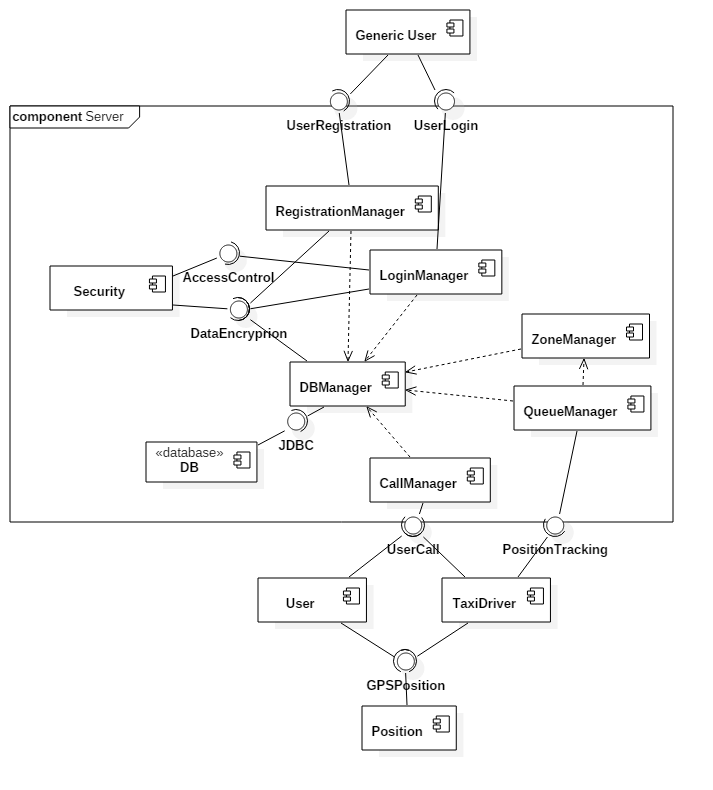
\includegraphics[width=12cm]{./Images/ComponentDiagram.png}
    \caption{Component Diagram of our system}
    \label{fig:component-diagram}
\end{figure}

\subsubsection{Client}
We now list the components of the client according to their level by starting from the highest level:
\begin{itemize}
    \item WebManager: it manages the web interfaces on the client side.
    \item AppManager: it manages the application on the client side.
    \item Generic user: it is formed of the functions that are in common between the passenger and the taxi driver.
    \item Passenger: it contains classes and functions concerning the passengers.
    \item Taxi: it contains classes and functions concerning the taxi drivers.
    \item Position: responsible for tracking the position of passengers and taxi.
\end{itemize}
These components have been deeply described in the DD.

\subsubsection{Server}
We now list the components of the server according to their level by starting from the highest level:
\begin{itemize}
    \item Registration Manager: responsible for the registration phase of a guest.
    \item Login Manager: responsible for the login phase, whether the user is a taxi driver or a passenger.
    \item Zone Manager: it manages the zones of the city.
    \item Queue Manager: it manages all the queues in which the city is divided into.
    \item Call Manager: responsible for managing the calls of passengers.
    \item DB Manager: it manages the interaction with the database.
    \item Security: responsible for granting the security to all the system.
\end{itemize}
These components have been deeply described in the DD.

\subsubsection{Database}
In this subsystem we have not identified any components because we do not have to develop this part; we assume that the database has been already tested and it need only to be integrated with the system.





